CAD é a sigla para "computer-aided design", design auxiliado por computador, e pode ser definido como o uso de sistemas
computadorizados (hardware + software) para criação, modificação, análise ou otimização do design
\cite{computer_aided_esign}.
O software CAD consiste em um programa capaz de implementar gráficos computadorizados e aplicar funções como análise
tensão-deformação de componentes, resposta dinâmica de mecanismos, cálculos de transferência de calor. As aplicações
variam conforme a necessidade da área.

\subsection{AutoCAD}
O software AutoCAD foi criado em 1982. Seu uso mais popular é em desenhos arquitetônicos, mas também é comumente
empregado na criação de desenhos técnicos.

\begin{figure}[h]
	\centering
	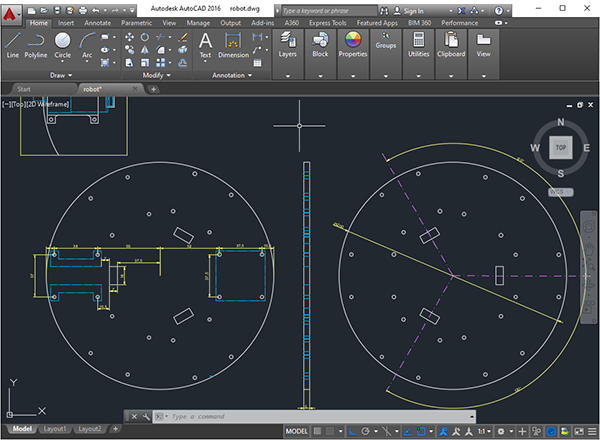
\includegraphics[width=1\textwidth]{figures/autocad_screen}
	\caption{Interface do AutoCad}
	\label{fig:interface_autocad}
\end{figure}

\subsection{SolidWorks CAD 3D}
Com um foco maior em projetos de engenharia, O SolidWorks é um  software CAD com foco na criação do modelo 3D de peças,
considerando precisão de medidas e materiais. O pacote de softwares adicionais oferece simulações de elementos finitos
como análise térmica, de vibrações, quedas, dinâmica, pressão, entre outros.

\begin{figure}[h]
	\centering
	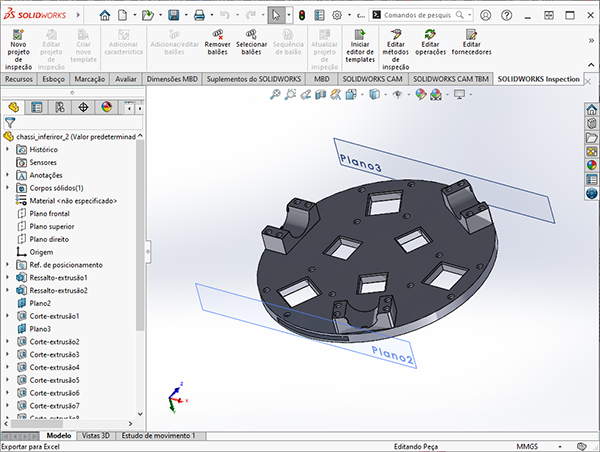
\includegraphics[width=1\textwidth]{figures/soliworks}
	\caption{Interface do SolidWorks}
	\label{fig:interface_soliwoks}
\end{figure}